%%%%%%%%%%%%%%%%%%%% author.tex %%%%%%%%%%%%%%%%%%%%%%%%%%%%%%%%%%%
%
% sample root file for your "contribution" to a contributed volume
%
% Use this file as a template for your own input.
%
%%%%%%%%%%%%%%%% Springer %%%%%%%%%%%%%%%%%%%%%%%%%%%%%%%%%%


% RECOMMENDED %%%%%%%%%%%%%%%%%%%%%%%%%%%%%%%%%%%%%%%%%%%%%%%%%%%
\documentclass[graybox]{svmult}

% choose options for [] as required from the list
% in the Reference Guide

\usepackage{type1cm}        % activate if the above 3 fonts are
                            % not available on your system
%
\usepackage{makeidx}         % allows index generation
\usepackage{graphicx}        % standard LaTeX graphics tool
                             % when including figure files
\usepackage{multicol}        % used for the two-column index
\usepackage[bottom]{footmisc}% places footnotes at page bottom


\usepackage{newtxtext}       % 
\usepackage{newtxmath}       % selects Times Roman as basic font

% see the list of further useful packages
% in the Reference Guide

\makeindex             % used for the subject index
                       % please use the style svind.ist with
                       % your makeindex program

%%%%%%%%%%%%%%%%%%%%%%%%%%%%%%%%%%%%%%%%%%%%%%%%%%%%%%%%%%%%%%%%%%%%%%%%%%%%%%%%%%%%%%%%%

%=========================Manage Comments=============================
\usepackage{color}
\usepackage{ifthen}
\newboolean{showcomments}
\setboolean{showcomments}{false} % toggle to show or hide comments
\ifthenelse{\boolean{showcomments}}
    {
        \newcommand{\emelie}[1]{\textcolor{red}{{\it [Emelie says: #1]}}}
        \newcommand{\peggy}[1]{\textcolor{blue}{{\it [Peggy says: #1]}}}
        \newcommand{\per}[1]{\textcolor{cyan}{{\it [Per says: #1]}}}
        \newcommand{\othercomment}[1]{\textcolor{magenta}{{\it [#1]}}}
    }
    {
        \newcommand{\emelie}[1]{}
        \newcommand{\peggy}[1]{}
        \newcommand{\per}[1]{}
        \newcommand{\othercomment}[1]{}
    }
%=======================================================================

%(1)    The formatting templates (in both LaTeX and Word) are available under [1]. The current LaTeX template is directly available at [2] (please use the template from the subdirectory “author” in the zip file) and the current Word template at [3].
%(2)    The chapters should be written in a clear, consistent, self-contained textbook-like style. Therefore, please comply with the following structure:
%a.       Each chapter should start with an “Introduction” and end with a short “Conclusion”. Please also consider a section “Recommended Further Reading” before the Conclusion.
%b.       The goal of each chapter is to give a comprehensive overview on a contemporary topic in empirical software engineering (for your convenience you find below a list of the confirmed chapter topics)
%c.       Please provide examples and evidence
%(3)    The intended length of your chapter should be approximately 25 pages.
%(4)    The deadline to submit the first version of the chapter is the 30th of April 2019.



\begin{document}

\title*{The Design Science Paradigm as a Frame for Empirical Software Engineering}
% Use \titlerunning{Short Title} for an abbreviated version of
% your contribution title if the original one is too long
\author{Per Runeson, Emelie Engstr\"om and Margaret-Anne Storey}
% Use \authorrunning{Short Title} for an abbreviated version of
% your contribution title if the original one is too long
\institute{Per Runeson and Emelie Engst\"om \at Lund University, Sweden, \email{[per.runeson;emelie.engstrom]@cs.lth.se}
\and Margaret-Anne Storey \at University of Victoria, Canada, \email{mstorey@uvic.ca}}
%
% Use the package "url.sty" to avoid
% problems with special characters
% used in your e-mail or web address
%
\maketitle
\abstract*{Each chapter should be preceded by an abstract (no more than 200 words) that summarizes the content. The abstract will appear \textit{online} at \url{www.SpringerLink.com} and be available with unrestricted access. This allows unregistered users to read the abstract as a teaser for the complete chapter.
Please use the 'starred' version of the \texttt{abstract} command for typesetting the text of the online abstracts (cf. source file of this chapter template \texttt{abstract}) and include them with the source files of your manuscript. Use the plain \texttt{abstract} command if the abstract is also to appear in the printed version of the book.}

\abstract{Software engineering research aims to contribute to improved real-world practice. With the adoption of empirical software engineering research methods, the understanding of real-world needs and evaluation of proposals has evolved, while a systematic approach to design or improvement is less advanced in the community.   The \emph{design science paradigm} offers a frame for software engineering research, embracing both improvement and evaluation in its constituents of \emph{problem understanding, solution (or artefact) design}, and \emph{evaluation}, with the practical recommendations phrased as \emph{technological rules}. We elaborate these constructs, with a focus on software engineering, relate them to different conceptualizations of design science, and provide examples of research methods to be used. We outline how both industry-academia communication and theoretical knowledge building may be supported by the design science paradigm, and provide examples of software engineering research, presented through a design science lens.} 

\section{Introduction}
\label{sec:intro}

\begin{itemize}
\item Software engineering research aims at practically useful methods, technologies and tools to help industry to improve software engineering practice. 
\item Discussed already when SE was defined \emph{The phrase 'software engineering' was [...] implying the need for software manufacture to be based on the types of theoretical foundations and practical disciplines, that are traditional in the established branches of engineering} \cite[p13]{Nato1968}.
\item Lots of solution proposals have been published, be it development methods/processes, tools, languages, although not evaluated in large scale SE.
\item With the advent of empirical SE, focus shifted towards validation of solution proposals. 
\item Families of experiments, systematic literature reviews, theory building to systematically add to the knowledge basis.
\item GQM, QIP, ... as improvement methods
%\item Industry-academia collaboration -- methods, models -- aim to make research more relevant 
%\item Continuous* for engineering cycles -- applicable for research?
\item The Design Science paradigm integrates \emph{problem understanding, solution design and evaluation} Functions as a context for ESE.
%\item Action research/technical action research -- research methods to impact practice
\item Different methods can be used within the DS paradigm
\end{itemize}

\section{Design Science -- an overview}
%Design science is a paradigm not a method}
\begin{itemize}
\item Introduction of DS concepts/constructs
\item Introduction of DS as a paradigm
\item Introduction of VA as a template
\item Specifics of SE as DS
\end{itemize}

\subsection{Design Science Constructs}

Design science is a \emph{paradigm}, that helps framing research, aiming towards improving an area of practice. In our case, the engineering of software is the practice area in focus. The practice is not homogenous over all kinds of software engineering, neither are the potential improvements the same for all instances of practice. Thus, design science addresses a general problem by studying  specific \emph{problem instances}, which constitute the research context where the research activities of \emph{problem understanding}, \emph{solution design} and \emph{evaluation} take place. \per{Activites -- leading too much towards method?}\emelie{no I think is is ok, but how does the validation of the TR relate to these activities?}

Design science does not prescribe a specific methodology nor specific method steps to be conducted in a single research study. The above mentioned activities are constituents of  a research process, that may be instantiated in different ways. Different methodologies -- empirical, analytical, and  design methodologies -- may be used within the frame of design science. Further, a single study or research paper may or may not contain all the constituents of the design science paradigm; one study may be focused on, for example,  problem understanding only\emelie{but not all exploratory studies provide design knowledge}\per{agree, but will make that distinction later in the chapter}, another may report the complete chain from problem identification to evaluated solution. Studies focusing on one aspect of design science may contain research contributions that build on or constitute basis for other research under the design science paradigm.

%Technological rules
The scientific knowledge, emanating from design science research, is typically captured in \emph{technological rules}. This means ``field-tested and grounded'' examplars of how a problem can be solved~\cite{van_aken_management_2004}. A technological rule is typically expressed in the following form: 

\begin{quote}{To achieve <effect/change> in <situation/context> use/apply <solution/intervention>}\end{quote}

As an example, a technological rule, summarizing the scientific knowledge from our paper on automated assignment of bugs to teams \cite{JonssonBug15}, can be phrased as:
\begin{quote}{To achieve more effective assignment of bugs to teams in large scale industrial contexts use ensemble-based machine learning to automate bug assignment. \cite{StoreyESEM17}}\end{quote}

Technological rules may be defined at different levels of abstraction... \per{Open up for more elaborate discussion below.}


% Problem understanding
Design science research aims to address real practice problems, and thus \emph{problem understanding} is a core constituent of the research. There is a large battery of empirical methods available for problem understanding -- case studies \cite{Runeson12Case}, surveys, data mining \cite{MenziesDataMining2016}, ethnography studies \cite{SharpEthnography2016}, etc. -- that can be used for the purpose.

Problem understanding is typically, but not necessarily, the first step in a design science research endeavor.\emelie{at least in an engineering endeavour, not sure about this ... We claim that the researchers role is not mainly to design solutions to specific problems but to provide generic prescriptions for practitioners to apply in their contexts} \per{Still, the design knowledge is gained through a particular instance. Added:}Understanding a general problem, present in one or more concrete problem instances, is a basis for understanding how this general problem may be solved.  While exploring a specific problem instance,   it may become clearer what the core of the problem is, and thus focussing the potential solution design to these areas. 

%\emelie{the problem needs to be described in terms of the envisioned solution} \per{added}
While problem understanding is a basis for the research activity, it is not a pure description of the problem. The problem needs to be described in terms of the envisioned solution. Researchers take a perspective on the problem at hand, which is colored by their knowledge and experience. A behavioral scientist would make different a different problem description of a software project, compared to a software engineering scholar, and different software engineering researchers are influence by their background as well. This implies that the problem understanding is intertwined with the solution design.

% Solution design
The outcome of a design science research endeavor is ultimately that \emph{design knowledge} is produced, that is, knowledge about how to design solutions to specific problems. The knowledge is gained while solving the identified problem at hand, and abstracted as general knowledge. Wieringa describes design science as an act of producing knowledge by designing useful things~\cite{wieringa_design_2009}.  Van Aken describes the typical design science strategy to be the multiple case study~\cite{van_aken_management_2004}, which can be compared with clinical research alpha- and beta testing, i.e. first case and succeeding cases. This emphasizes the need for replication studies to validate design knowledge. \per{Discussion on artifact vs design below.}

The solution aims to address a specific problem instance, and has hence to be designed in that context, However, design knowledge can be generalized from that context, either if the design artefact itself is general enough to fit other contexts, or of the design methodology can be applied in another context.
\per{Something more on design approach?}

% Evaluation
The \emph{evaluation} \emelie{should we use the term validation instead} \per{The VA says evaluation}in design science research focuses on the \emph{problem--solution pair}. The primary goal is to assess whether the solution proposal is feasible for the problem instance. However, the scope of the design knowledge gained, can be extended by systematically extending the scope of the evaluation.  Stol and Fitzgerald adapted McGrath's framework for research strategies, to guide balancing generalizability, precision and realism in designing evaluation studies \cite{StolABC18}.


%Design Science as a Lens
We analyzed of software engineering literature from a design science perspective, \per{Could we mention the ICSE study? We may put the manuscript in arXiv when it is submitted}and concluded that the design science paradigm is not explicitly used as a frame for the research, although the constructs of design science research are present implicitly. Thus, we designed a \emph{visual abstract template} to help identifying the design science constructs in software engineering research \cite{StoreyESEM17}, see Figure~\ref{fig:VA-template}. 

Our DS template covers the main constructs of DS research: The theoretical contribution in terms of a \emph{technological rule}; its instantiation in terms of a real \emph{problem-solution} pair;  the empirical or theoretical support for the \emph{problem} understanding, the \emph{solution} design. Further, the bottom three boxes address the relevance of the research, the rigor of the research activities, and a statement what is novel in relation to the underpinning research, be it the problem udnerstanding, the solution design, or the validation of the problem--solution pair in a new instance.
\begin{figure*}
% Use the relevant command to insert your figure file.
% For example, with the graphicx package use
  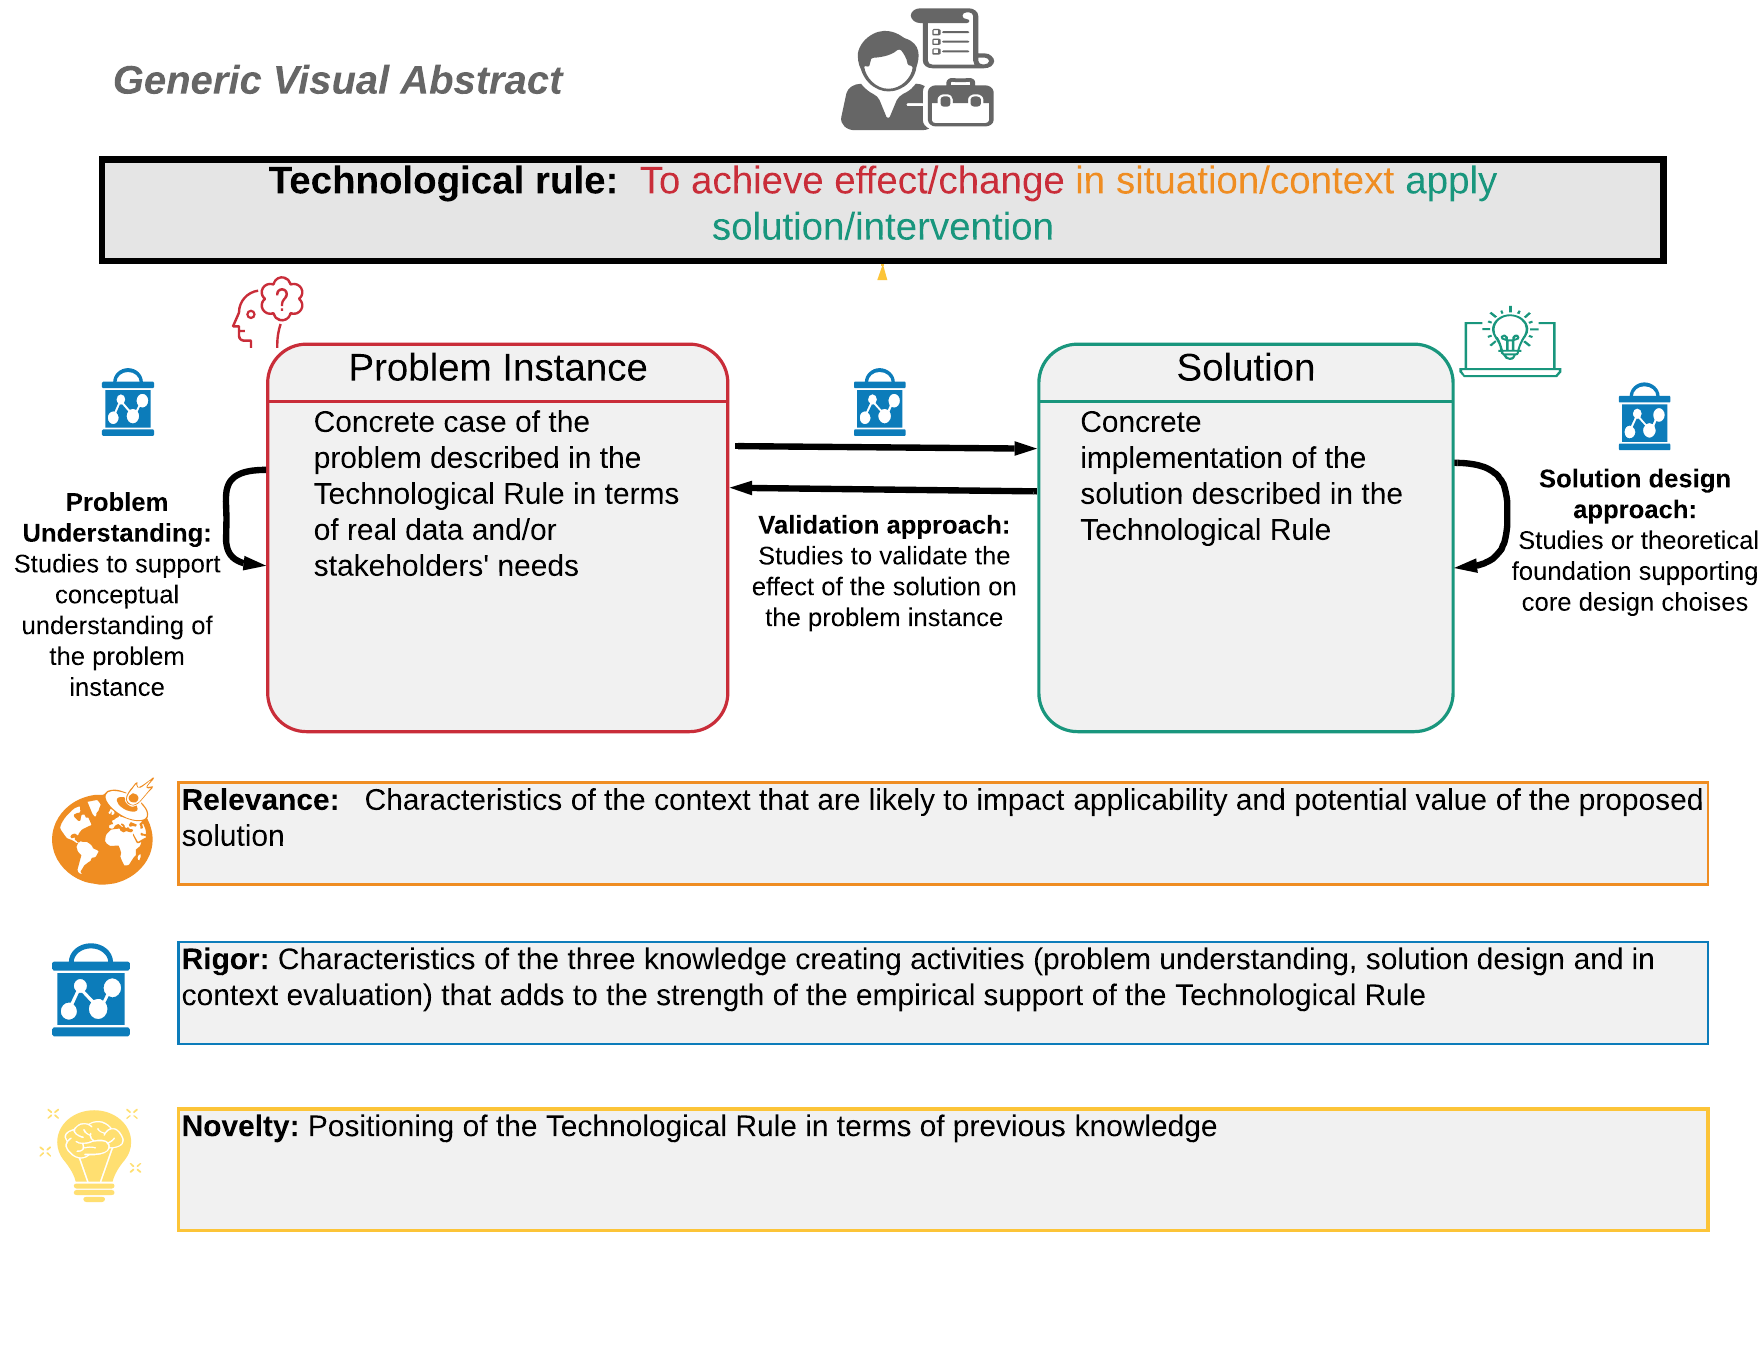
\includegraphics[width=1.0\textwidth]{Figures/GenericVA.png}
% figure caption is below the figure
\caption{Visual abstract template including the core constructs in design knowledge}
\label{fig:VA-template}       % Give a unique label
\end{figure*}

Design science is a paradigm used in many different research fields, and there are many variants of the instantiation. The above summary reflects what we have found suitable in software engineering, and some of our rationale and alternative instantiations are discussed in the elaborated section below.


\subsection{Design Science is a Paradigm}
Design science is a research paradigm and as such it contains a set of beliefs regarding both the type and nature of knowledge as well as on how it can be validated. Although none of the design science advocates in the software engineering community would disagree with this claim, design science is often discussed as if it was a specific methodology to be selected among other empirical methods. 

The philosophical stance behind design science is what is characterized as pragmatism~\cite{easterbrook_selecting_2008}\emelie{it is a philosophical tradition from 1870 not sure what reference to use...}, referring to a view that all knowledge is approximate and valued by its usefulness for solving practical problems. Hevner et al. express this in terms of utility: 

\begin{quote}
	``If the artifact does not solve the problem (search, implementability), it has no utility. If utility is not demonstrated (evaluation), then there is no basis upon which to accept the claims that it provides any contribution (contribution).''~\cite{hevner_design_2004}
\end{quote}\emelie{check quote} 

Pragmatists strive to reach consensus over evidence, why access to stakeholders' perceptions are necessary in the validation of design knowledge. Since such stance is less dogmatic than other philosophical stances, our emphasis when applying the design science lens, is on the type and nature of the produced knowledge rather than on the methodology applied. Various methods may be used to gain insights into a problem.

Gregor and Hevner refer to design science as a paradigm~\cite{gregor_positioning_2013}. Johannesson, on the other hand, disagrees with this and argues that design science refers to the objective of changing the world, in contrast to describing it, and that this is done primarily by creating artefacts not knowledge~\cite{johannesson_introduction_2014}. Our stance is that design science is a paradigm for software engineering research and as researchers our primary goal is to create knowledge to be applied by practitioners in the field. Furthermore, we consider artefacts as embedding knowledge. 


%\paragraph{Design science is more than action research.}

Another example of using the design design science lens on a problem domain similar to software engineering is van Akens' proposal to distinguish management theory, that is prescriptive, from organisational theory, that is explanatory~\cite{van_aken_management_2005}. He focuses on the product of the research process, i.e. design knowledge, rather than research it self and introduces the notion of technological rules as being field-tested and grounded solution-oriented knowledge. 

Action research is one way of producing and validating technological rules but it is not the only way. Action research does not explicitly aim at developing valid knowledge that can be transferred to other contexts but rather to make a change in one specific local context. Both Wieringa~\cite{wieringa_technical_2012} and Johannesson~\cite{johannesson_introduction_2014} discuss action research as one of several empirical methods that can be used to produce design knowledge.


\begin{figure*}
% Use the relevant command to insert your figure file.
% For example, with the graphicx package use
  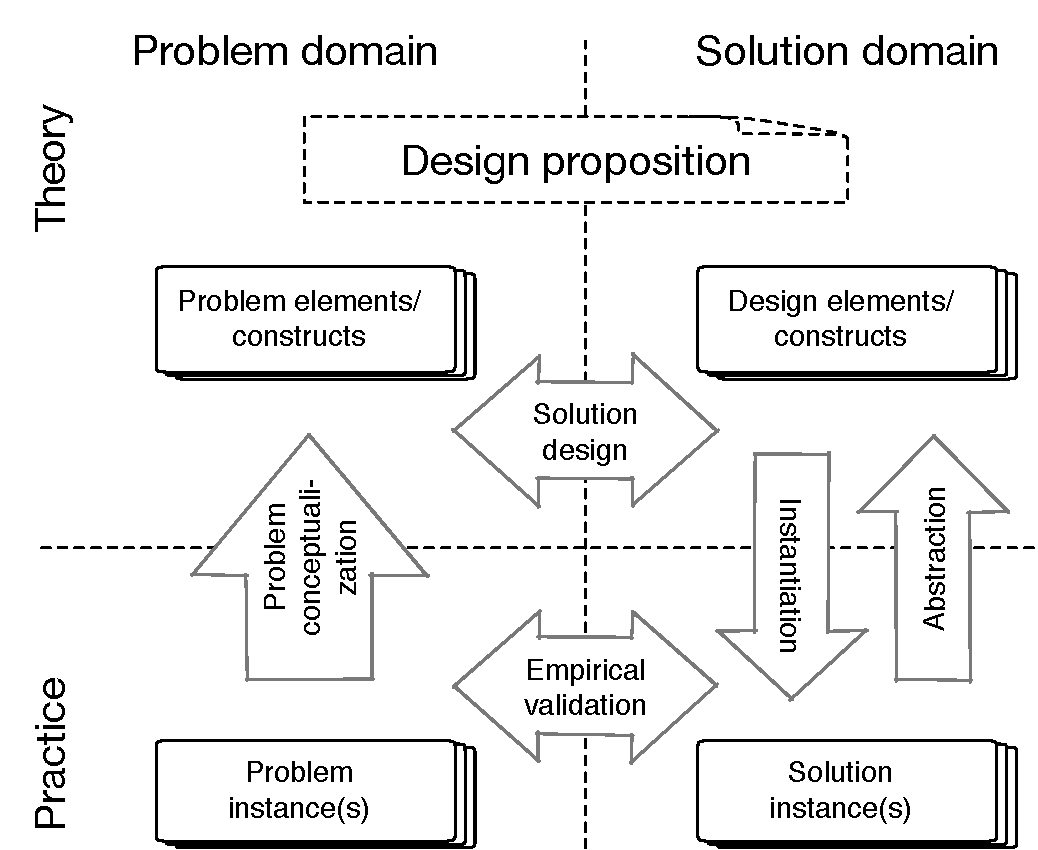
\includegraphics[width=0.75\textwidth]{Figures/DS_model.pdf}
% figure caption is below the figure
\caption{Contribution types in design science research}
\label{fig:contributiontypes}       % Give a unique label
\end{figure*}

%Compare to action research and other empirical methodologies case studies and experiments.


\subsection{Software Engineering Research as Design Science}
\begin{itemize}
\item Paper example Jonsson \cite{JonssonBug15} from \cite{StoreyESEM17}, or something different.
\item Method examples? Gorschek? \cite{GorschekSW2006}
\item Units of research -- not necessarily one paper/study.
\end{itemize}

\paragraph{The design science lens provides a holistic view on a research contribution.} 

Any design science research contribution should be viewed in its context, which includes both a problem formulation and a solution proposal and, in case of an empirical contribution, instances of both, see Figure~\ref{fig:contributiontypes}. Thus a problem conceptualisation must be presented in terms of the envisioned solution, and a solution evaluation in terms of the problem formulation. 
Just like Gregor and Hevner~\cite{gregor_positioning_2013}, Wieringa emphasises that it is the artefact in context being the object of study in design science~\cite{wieringa_design_2009}.

\section{Technological rules}
\begin{itemize}
\item Definition
\item Theoretization
\end{itemize}

\subsection{Design knowledge generalised to technological rules}
%\subsubsection{Design knowledge is prescriptive and context dependent.} 
In line with van Akens proposal~\cite{van_aken_management_2004}, we describe design knowledge in terms of technological rules. Such rules comprise both the context in terms of the \emph{desired effect} and \emph{the situation} and a prescription in terms of a \emph{proposed solution or intervention}. see Figure~\ref{fig:VA-template}. Furthermore we argue that technological rules can be expressed at any convenient abstraction level and that they are hierarchically related to each other. However, TRs expressed at a very high abstraction level (e.g. "To produce software of high quality apply good software engineering practices") tend to be either trivial or too bold (easy to debunk) while rules at very low abstraction levels have a narrow scope and thus lack relevance for most software engineers. Thus it is important to explicitly formulate the technological rule when presenting design science research and to be consistent with it both when arguing for its relevance and its novelty as well as when presenting the empirical (or analytical) support for the claims. 

Hevner et al. do not emphasise generality of the contribution as such but consider the instances of problems-artefact-utility as the research contribution. Instead generalisability or external validity is discussed as a quality attribute of such contribution~\cite{hevner_design_2004}. Gregor and Hevner, on the other hand do put forward design theory as the result of generalising from a problem instance to a class of problems and defining the scope of validity of a solution~\cite{gregor_positioning_2013}. Also Wieringa discusses design theory, defining it as theories of artefacts in context~\cite{wieringa_design_2009}. Wieringa and Daneva address generalisability of design theory ~\cite{wieringa_six_2015} and argue that there is no such thing as general design theories, instead they emphasise the utility of middle-ranged theory, defined as theories lacking universal scope. One could argue that useful technological rules are such middle-ranged theory constructs.

\subsection{Maturation of technological rules}
\paragraph{Technological rules mature through increments of problem understanding, solution design and evaluation of the solution applied to the problem} 

Design knowledge is gained through studying real-world problem-solution pairs. We agree with Wieringa that we cannot provide evidence for general design theory~\cite{wieringa_six_2015}. Still, general technological rules are the actionable outcome of our research and should be formulated (without evidence). However, of course we may and should provide empirical and analytical support for the technolgical rules we put forward. van Aken describes the typical design science strategy to be the multiple case study~\cite{van_aken_management_2004}, which could be compared with clinical research alpha- and beta testing, i.e. first case and succeeding cases. We agree with this and stress the need to study the real world instance of the problem and the implementation of the solution as a whole.

\section{Problem understanding}
\begin{itemize}
\item Problem instance
\item Empirical observations of practice
\item Literature as a sources of problem understanding?
\end{itemize}


\paragraph{Problem understanding is dependant on the envisioned solution.}Although we consider much of the software engineering research to be design science research, in that its uttermost goal is to provide well-informed recommendations to practitioners, not all exploratory and descriptive research provide relevant design knowledge. In order for the exploratory and descriptive knowledge to be considered design knowledge it must be described in terms of the solution to be designed. This is illustrated in Figure~\ref{fig:contributiontypes}. If for example the proposed solution is to design a visualisation system, the problem should typically be described in terms of a group of target users, their questions, and their measurements or data~\cite{meyer_nested_2015}. \emelie{I'm not sure the papers in our descriptive/problem cluster passes this criteria}

\per{A solution searching the problem?}

\paragraph{Software engineering design problems are socio-technical}
Problems are described as improvement problems and/or construction problems, wicked problems, socio-technical, involving stakeholders. 



\section{Solution design}
\paragraph{Design science is more than artefact design.}

Design science comprises both creation and validation of design knowledge, i.e. prescriptive and context dependant knowledge. Such knowledge can be achieved by investigating real world instances of problem-solution pairs. We have identified three different knowledge creating activities of which the \emph{solution design} is one. The other two are the \emph{problem understanding} and the \emph{empirical evaluation} of the solution to the problem in context, see Figure~\ref{fig:VA-template}.

Wieringa describes design science as an act of producing knowledge by designing useful things~\cite{wieringa_design_2009} and makes a distinction between knowledge problems and practical problems. Similarily, Gregor and Hevner emphasise the dual focus on the artefact and its design~\cite{gregor_positioning_2013} in information systems, and argues for an iterative design process where evaluation of the artefact provides feedback information to improve both the design process and the artefact. Although such an approach may be relevant for designing software engineering artefacts too, there is an important difference between the two research domains: while information systems refers to a solution domain, software engineering research originates in a problem domain with a plethora of more or less sophisticated solutions, not necessarily artefacts. Thus the empirical contribution to problem understanding is of higher importance in the software engineering context while the reflection on the design as such is of less value compared to research contributions in a typical solution domain such as information systems. Still, in both cases it is design knowledge that is produced as the aim is to produce prescriptive knowledge for practitioners in their respective domain. 

\paragraph{Solution design is constituted by a set of important design decisions.}  The actual design of a real-life solution is the act of the practitioner, preferably guided by design knowledge produced by researchers. However, one activity to produce design knowledge is to work though increments of a solution design either together with practitioners in a real-life setting or off-line. To make the design knowledge accessible and trustworthy, critical design decisions of a solution design activity carried out by researchers should be clearly reported, together with considerations about alternative solutions. 

\paragraph{Software engineering solutions can be described as interventions to the software development process}
Solutions are described as interventions/artefacts and prescriptions



\section{Evaluation}
\begin{itemize}
\item Problem--solution pair \emph{in context}
\item Widening scope by widening evaluation context. 
\item theoretical/analytical generalization rather than statistical 
\item All kinds of empirical studies \cite{easterbrook_selecting_2008}\cite{Runeson12Case,WohlinExpBook12}
\item Refer to ABC \cite{StolABC18} for strategic choise of method vs evaluation goal
\end{itemize}



Design science has been conceptualised by several researchers in software engineering and other disciplines, such as information systems~\cite{gregor_positioning_2013}. Our conceptualisation that is presented in this paper and on which our analysis is based have been formed through a thorough review of this literature and a series of workshops on the topic. Below we position our view of design science in software engineering.



\section{Using the Design Science Frame in Software Engineering}
We see three direct uses of the design science paradigm as a frame for software engineering research. Firstly, it can help assessing contributions in research, both in the research community and during planning and design of research (Section \ref{sec:assessment}). Secondly, design science, particularly the technological rule, can be used in knowledge building, advancing the theoretical knowledge in the software engineering field (Section \ref{sec:knowledge}). Thirdly, the design science frame may help communicating research within the community and with industry (Section \ref{sec:communication}).

\subsection{Assessment of contributions}
\label{sec:assessment}
\paragraph{Evaluation should be made in context and test the impact of the solution on the real problem}

\subsubsection{Relevance of a design science study is described in terms of problem similarity and solution applicability.} The relevance of a research contribution could be viewed from two perspectives, the targeted practitioners and the research community. From the individual practitioner's point of view the relevance of a research contribution is assessed by comparing their specific context with the one described in the research report. From the research community on the other hand a measure of relevance is often requested in terms of how common the studied problem is. To enable both types of assessments relevant context factors need to be reported. Not all context factors are helpful in making this assessment but only those that are critical for either the applicability of the solution or for the potential gain of applying the solution. 


\subsubsection{Rigor of a design science study refers to the strength of the added support for the technological rule.} Rigor may be assessed in all of the three knowledge creating activities. However, the solution design activity is by nature a creative process and does not necessarily add to the rigor of the study. One aspect of rigor in the design activity could be the extent to which it is built on prior design knowledge. Also the consideration of alternative solutions could be taken in to account. The other two activities, i.e. problem understanding and solution evaluation, are on the other hand based on common empirical methods on which relevant validy criteria can be applied. 

\subsubsection{Novelty of a design science study is expressed in terms of new or refined technological rules.} Technological rules may be expressed at several abstraction levels, thus it is always possible to identify an abstraction level at which a research contribution is novel, may it be at the cost of general relevance. To optimise rigor, novelty and relevance of reported research, the researchers should strive to express the technological rule at the highest possible abstraction level, at which it is novel, the provided evidence give strong support and are not debunked by previous studies (or common sense). However, adding empirical support for existing, but under-evaluated, technological rules have a value of its own, which makes novelty less important than the rigor and relevance criteria.


\subsection{Knowledge building}
\label{sec:knowledge}

\begin{itemize}
\item Technological rule -- as a means for knowledge summary
\item Theory building
\item Continuous learning and improvement
\item Generalization
\end{itemize}

\subsection{Research communication}
\label{sec:communication}

\begin{itemize}
\item Technological rule -- as a means for communication
\item Visual abstracts
\end{itemize}

\cite{CarverIEEESW2018}

\section{Examples}
Either we choose examples that illustrate the different aspects of DS, or we choose three examples that are good examples of DS -- candidates from the ICSE best papers, or our own papers?



\section{Recommended Further Reading}

Hevner has conceptualized design science for information systems research, combining behavioral science and design science research \cite{hevner_design_2004,hevner_design_2010}.

Van Aken explored the design science paradigm for management science, with a focus on theoretical contributions, captured as technological rules \cite{van_aken_management_2004,van_aken_management_2005}. 

Wierenga instantiated design science for software engineering and information systems research in the concept of technical action research, including an engineering cycle and an empirical research cycle \cite{wieringa_design_2009,wieringa_six_2015,wieringa_technical_2012,wieringa_what_2014}.

Johannesson? \cite{johannesson_introduction_2014}.

\section{Conclusion}

%\tableofcontents


\bibliographystyle{plain}
\bibliography{dsse}
\end{document}
